\chapter{State of the Art}\label{cap:estadoDeLaCuestion}

In this chapter, we present the fundamental concepts underlying the design of our chess engine, including the minimax search algorithm and alpha-beta pruning. We also explain how chess engines communicate through the Universal Chess Interface (UCI) protocol and discuss the Elo rating system, which is commonly used to evaluate the skill level of chess players. Additionally, we provide an overview of the \textit{Stockfish} engine, highlighting its architecture and the integration of machine learning techniques into its search algorithm. Finally, we describe several tools widely used in the chess programming community for debugging and evaluating engine performance.


\section{Game trees}

\par Two-player turn-based games, such as chess or tic-tac-toe, where players take alternating turns, can be represented using a game tree or graph. In this representation, the root node corresponds to the initial position from which we begin searching for the best move. Each subsequent node represents a possible game state resulting from a legal move, forming a branching, tree-like structure.

\vspace{1em}

\par The depth of the tree refers to the number of turns (or plies) from the root node to a leaf node, alternating between white and black. A ply refers to a single move made by one player. One ply corresponds to one move by either white or black, while a full turn (both players moving) consists of 2 plies. Deeper nodes represent positions further into the future of the game. A depth of 1 includes all possible moves for the current player (the side to move), while a depth of 2 includes the opponent's responses to those moves. As the depth increases, the process continues to alternate between the two players at each level of the tree. This means that the number of nodes grows exponentially, making it computationally expensive to explore every possible state.

\vspace{1em}

\noindent In~\cref{fig:game-tree}, the shaded cluster of lines on the left represents the part of the game tree corresponding to previous moves leading up to the current position. From there, only a subset of possible continuations is drawn, illustrating the immense complexity of chess. Claude Shannon estimated that the number of possible chess games is around $10^{120}$, a value known as the \textit{Shannon number}~\cite{Shannon1950}. This astronomical figure makes it computationally infeasible to represent or analyze the entire game tree, motivating the use of search algorithms and pruning techniques to explore only the most relevant branches, which are explained in the following section.

\begin{figure}[t]
    \centering
    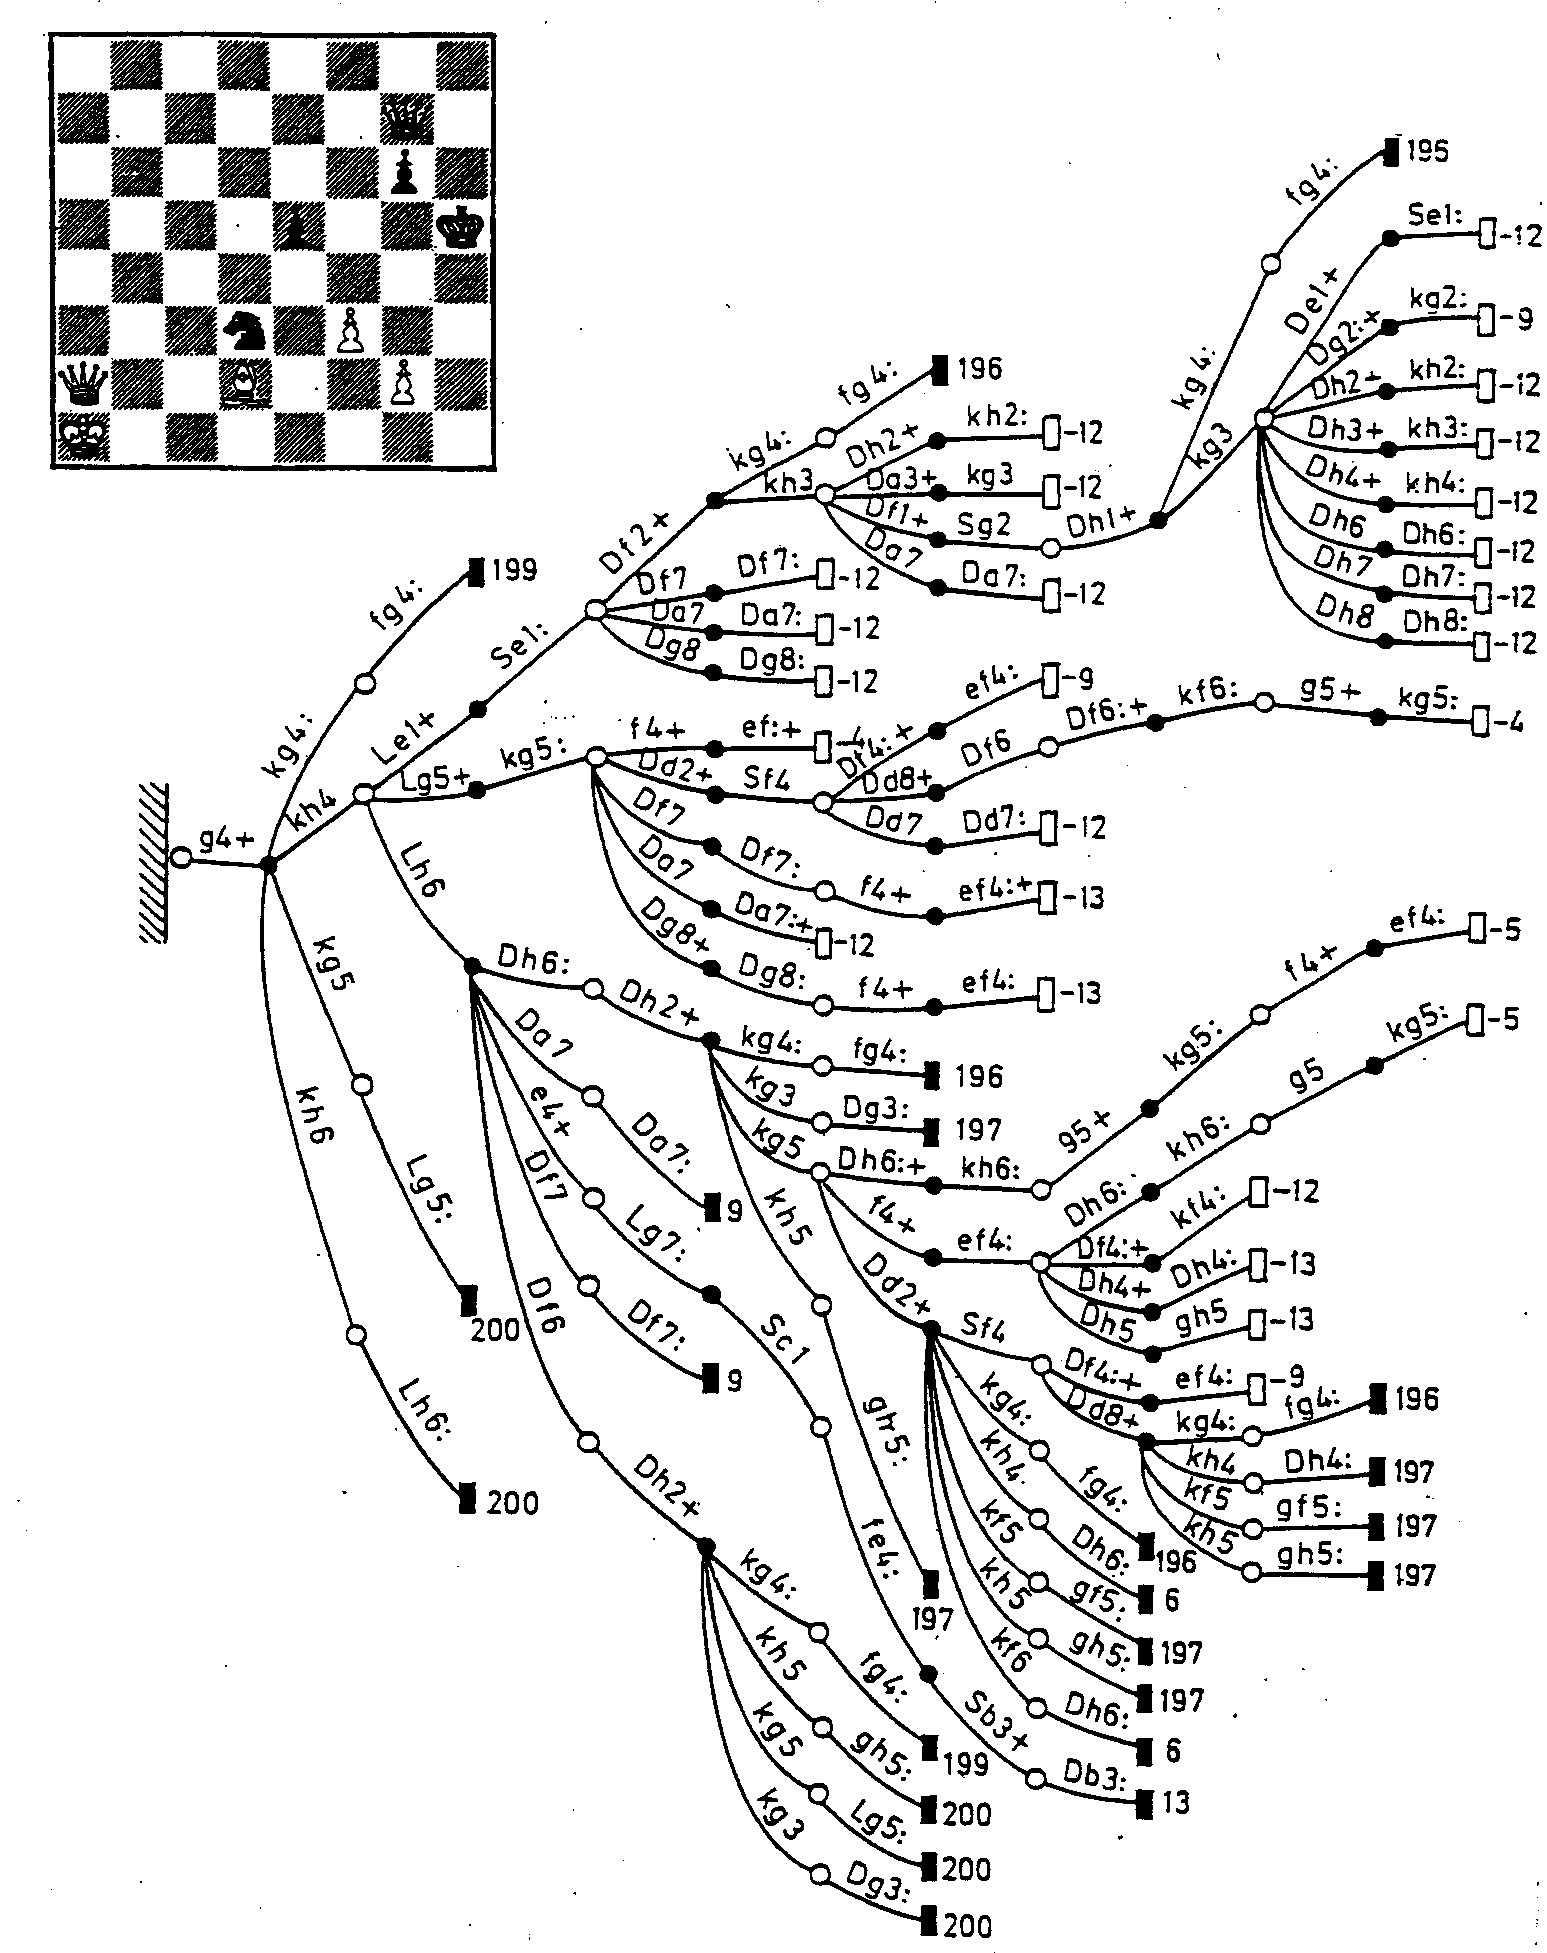
\includegraphics[width=0.5\textwidth]{Imagenes/chess-game-tree.jpg}
    \caption{Illustration of a game tree for a chess position~\cite{BotvinnikLongRangePlanning}.}\label{fig:game-tree}
\end{figure}

\section{Search algorithms}

There are different approaches to analyze and find the best move from a position. Some of these search algorithms are: Depth-First Search (DFS), Best-First Search (not to be confused with Breadth-First Search or BFS but they are related), and Parallel Search.

\vspace{1em}

\noindent Note that these search algorithms are the foundation of more advanced and practical algorithms used today. That is why explaining them is essential for understanding the underlying principles.

\paragraph{Depth-First Search} refers to the process of exploring each branch of a tree or graph to its deepest level before backtracking. Unfortunately, in chess, this cannot be possible as mentioned in the last section. This is because the number of possible moves grows exponentially with the depth of the search tree, leading to the so-called combinatorial explosion. To address this, depth-first search is often combined with techniques like alpha-beta pruning to reduce the number of nodes evaluated, making the search more efficient while still exploring the tree deeply.~\cref{lst:dfs} illustrates the working of the DFS algorithm.

\vspace{1em}

\begin{lstlisting}[caption={Pseudocode of the Depth-First Search algorithm~\cite{CLRS}.}, label={lst:dfs}, frame=single, numbers=left, xleftmargin=15pt, captionpos=b]
Procedure DFS(Graph G, Node v):
    Mark v as visited
    For each neighbor w of v in G.adjacentEdges(v):
        If w is not visited:
            Recursively call DFS(G, w)
\end{lstlisting}

\vspace{1em}

\noindent DFS visits nodes by marking them as visited (line 2) and recursively explores all adjacent nodes until no unvisited nodes remain (lines 3 to 5). It has a worst-case performance of $O(|V| + |E|)$ and worst-case space complexity of $O(|V|)$, with $|V| = \text{number of nodes}$ and $|E| = \text{number of edges}$.

\vspace{1em}

\noindent In practice, especially in chess, a bounded or depth-limited version of DFS is often used. In bounded DFS, the search is restricted to a maximum depth, preventing the algorithm from exploring the entire tree. This approach allows the algorithm to focus on the most relevant positions.

\paragraph{Best-First Search} refers to the way of exploring the most promising nodes first. It is similar to a breadth-first search but prioritizes some nodes before others. They typically require significant memory resources, as they must store a search space (the collection of all potential solutions in search algorithms) that grows exponentially.

\vspace{1em}

\begin{lstlisting}[caption={Pseudocode of the Best-First Search algorithm~\cite{Pearl1984}.}, frame=single, numbers=left, xleftmargin=10pt, breaklines=true, captionpos=b]
Procedure BestFirstSearch(Graph G, Node start, Node goal):
    Create an empty priority queue PQ
    Add start to PQ with priority 0
    Mark start as visited

    While PQ is not empty:
        Node current = PQ.pop()
        If current is the goal:
            Return the path to the goal

        For each neighbor w of current in G.adjacentEdges(current):
            If w is not visited:
                Calculate priority for w (e.g., using a heuristic)
                Add w to PQ with the calculated priority
                Mark w as visited
\end{lstlisting}

\vspace{1em}

\noindent In this case, the priority queue contains nodes along with their associated priorities, which are determined by a heuristic function. This process is commonly referred to as branch and bound, where the algorithm explores branches of the search tree according to their heuristic value.

\paragraph{Parallel Search} refers to mulithreaded search, a technique used to accelerate search processes by leveraging multiple processors.

\vspace{1em}

\noindent Next, we will discuss one of the most widely used search algorithms in chess engines: the minimax algorithm.

\subsection*{Minimax algorithm}\label{sec:minimax}

The \textbf{minimax} algorithm is a decision making algorithm that follows Depth-First Search (DFS) principles. It is based on the assumption that both players play optimally, with one player (the maximizer) trying to maximize his score and the other player (the minimizer) trying to minimize his score. It explores the game tree to evaluate all possible moves and determines the best move for the current player.~\cref{lst:minimax} has the pseudocode of the algorithm:

\vspace{1em}

\begin{lstlisting}[caption={Pseudocode of the Minimax algorithm~\cite{Russell2021artificial}.}, label={lst:minimax}, frame=single, numbers=left, xleftmargin=15pt, breaklines=true, captionpos=b]
Procedure Minimax(Node position, Integer depth, Boolean maximizingPlayer):
    If depth == 0 or position is a terminal node:
        Return the evaluation of the position

    If maximizingPlayer:
        Integer maxEval = -Infinity
        For each child of position:
            Integer eval = Minimax(child, depth - 1, False)
            maxEval = max(maxEval, eval)
        Return maxEval
    Else: // minimizingPlayer
        Integer minEval = +Infinity
        For each child of position:
            Integer eval = Minimax(child, depth - 1, True)
            minEval = min(minEval, eval)
        Return minEval
\end{lstlisting}

\begin{figure}[H]
    \centering
    \begin{tikzpicture}[
        level distance=1.5cm,
        level 1/.style={sibling distance=4cm},
        level 2/.style={sibling distance=2cm},
        circleNode/.style={circle, draw, minimum size=1cm, inner sep=0pt},
        squareNode/.style={rectangle, draw, minimum size=1cm, inner sep=0pt}
    ]
        % Root node
        \node[squareNode] (root) {3}
            child {node[circleNode] (b) {3}
                child {node[squareNode] (d) {3}}
                child {node[squareNode] (e) {5}}
            }
            child {node[circleNode] (c) {2}
                child {node[squareNode] (f) {2}}
                child {node[squareNode] (g) {9}}
            };

        \node[left=1.2cm] at (root) {MAX};
        \node[left=1.2cm] at (b) {MIN};
        \node[left=1.2cm] at (d) {MAX};

        % Edges
        \draw[-{Stealth}, draw=red] (b) -- (root);
        \draw[-] (root) -- (c);
        \draw[-{Stealth}, draw=red] (d) -- (b);
        \draw[-] (b) -- (e);
        \draw[-{Stealth}, draw=red] (f) -- (c);
        \draw[-] (c) -- (g);
    \end{tikzpicture}
    \caption{Example of minimax.}\label{fig:minimax}
\end{figure}

\noindent For example, let's say that white always wants the highest value (maximizing the result), while black wants the lowest value (minimizing the result). In~\cref{fig:minimax}, white is represented by square nodes and black by circle nodes. Note that this example is a binary tree, but in a real scenario there would likely be more moves or nodes, because in chess each position usually allows a wide range of legal moves, not just two as in a binary tree. For the leftmost pair of leaf nodes with values of 3 and 5, 3 is chosen because black tries to get the lowest score between them. Then, for the other pair of leaf nodes with values of 2 and 9, 2 is chosen for the same reason. Lastly, at the root node, white selects 3 as the maximum value between 3 and 2.

\subsection*{Alpha-beta pruning}\label{sec:alphaBeta}

Minimax has the problem that a lot of the node evaluation is redundant, because we can know beforehand that some branches will not affect the final decision. For that purpose, we can enhance the search with the \textit{alpha-beta pruning} technique. 

\vspace{1em}

\noindent Alpha-beta pruning is an optimization of the minimax algorithm that eliminates the need to explore parts of the tree that cannot influence the final decision. It maintains two parameters, \(\alpha\) and \(\beta\), which represent the best already explored option along the path to the root for the maximizer and minimizer, respectively.

\begin{itemize}
    \item \(\alpha\): the best value that the maximizer currently can guarantee.
    \item \(\beta\): the best value that the minimizer currently can guarantee.
\end{itemize}

During the recursive search:
\begin{itemize}
    \item At a maximizing node, we update \(\alpha = \operatorname{max}(\alpha, \text{value})\).
    \item At a minimizing node, we update \(\beta = \operatorname{min}(\beta, \text{value})\).
\end{itemize}

If at any point \(\alpha \geq \beta\), we can prune the remaining children of that node, as they will not affect the final decision.

\vspace{1em}

This technique can drastically reduce the number of nodes evaluated, especially if the best moves are searched first. In the best case, alpha-beta pruning reduces the time complexity from \(O(b^d)\) to \(O(b^{d/2})\), where \(b\) is the branching factor and \(d\) the depth of the tree.

\vspace{1em}

\noindent\cref{fig:alphaBetaExample} demonstrates the alpha-beta search process by using $alpha$ ($\alpha$) and $beta$ ($\beta$) values. First, we obtain the leftmost and deepest number, which is $3$, and $\beta$ is set to this number on the node above, representing the current lowest bound. Then, $3$ is compared with the following node on the same depth, $5$, and the MIN node selects the minimum value between $3$ and $5$, which is $3$. Next, this $\beta$ value is passed up to the MAX node above, updating its $\alpha$ value to $3$. This means that the upper bound for that node must be a number less than or equal to $3$. Then, the last calculated $\alpha$ value is passed to the MIN node in the right subtree. To determine its value, we continue down to the next depth, where the first node has a value of $2$. This value updates the $\beta$ value of the MIN node above, with the passed $\alpha$ value. Now, this MIN node can only take a value between $3$ and $2$, meaning the node with a value of $1$ cannot be a solution and is pruned.

\vspace{1em}

\noindent Throughout this process, branches that cannot possibly influence the final decision are pruned, significantly reducing the number of nodes that need to be evaluated. This demonstrates the efficiency of alpha-beta pruning in minimizing the search space while guaranteeing the same result as a full minimax search.

\begin{figure}[htbp]
    \centering
    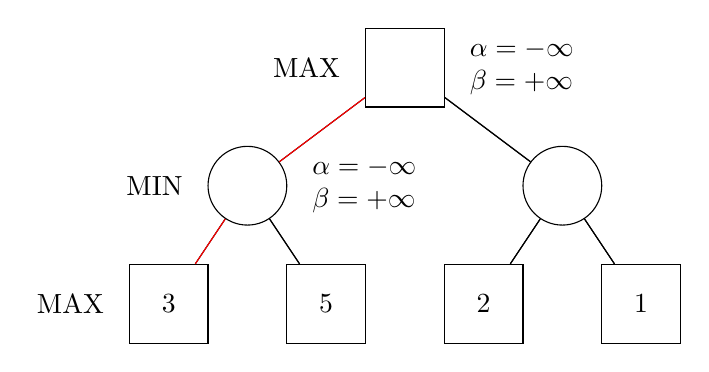
\begin{tikzpicture}[
        level distance=1.5cm,
        level 1/.style={sibling distance=4cm},
        level 2/.style={sibling distance=2cm},
        circleNode/.style={circle, draw, minimum size=1cm, inner sep=0pt},
        squareNode/.style={rectangle, draw, minimum size=1cm, inner sep=0pt}
    ]
        % Root node
        \node[squareNode] (root) {}
            child {node[circleNode] (b) {}
                child {node[squareNode] (d) {3}}
                child {node[squareNode] (e) {5}}
            }
            child {node[circleNode] (c) {}
                child {node[squareNode] (f) {2}}
                child {node[squareNode] (g) {1}}
            };

        % Labels for alpha and beta
        \node[right=0.7cm, align=left] at (root) {$\alpha = -\infty$ \\ $\beta = +\infty$};
        \node[right=0.7cm, align=left] at (b) {$\alpha = -\infty$ \\ $\beta = +\infty$};

        % Node labels
        \node[left=0.7cm] at (root) {MAX};
        \node[left=0.7cm] at (b) {MIN};
        \node[left=0.7cm] at (d) {MAX};

        % Edges
        \draw[-, draw=red] (root) -- (b);
        \draw[-] (root) -- (c);
        \draw[-, draw=red] (b) -- (d);
        \draw[-] (b) -- (e);
        \draw[-] (c) -- (f);
        \draw[-] (c) -- (g);
    \end{tikzpicture}
    \caption{Alpha-beta pruning - step 1}\label{fig:alphaBetaExample}
\end{figure}

\begin{figure}[htbp]\ContinuedFloat
    \centering
    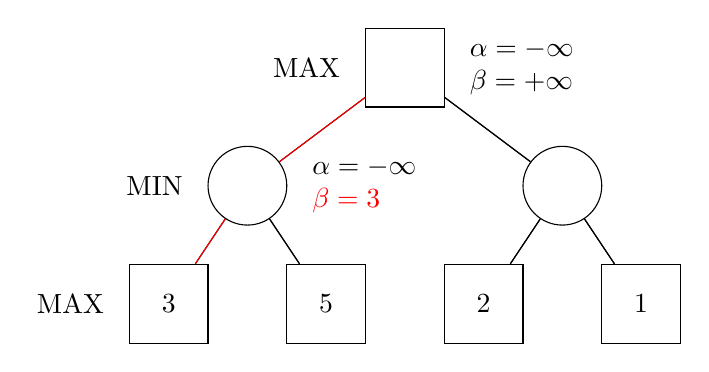
\begin{tikzpicture}[
        level distance=1.5cm,
        level 1/.style={sibling distance=4cm},
        level 2/.style={sibling distance=2cm},
        circleNode/.style={circle, draw, minimum size=1cm, inner sep=0pt},
        squareNode/.style={rectangle, draw, minimum size=1cm, inner sep=0pt}
    ]
        % Root node
        \node[squareNode] (root) {}
            child {node[circleNode] (b) {}
                child {node[squareNode] (d) {3}}
                child {node[squareNode] (e) {5}}
            }
            child {node[circleNode] (c) {}
                child {node[squareNode] (f) {2}}
                child {node[squareNode] (g) {1}}
            };

        % Labels for alpha and beta
        \node[right=0.7cm, align=left] at (root) {$\alpha = -\infty$ \\ $\beta = +\infty$};
        \node[right=0.7cm, align=left] at (b) {$\alpha = -\infty$ \\ $\textcolor{red}{\beta = 3}$};

        % Node labels
        \node[left=0.7cm] at (root) {MAX};
        \node[left=0.7cm] at (b) {MIN};
        \node[left=0.7cm] at (d) {MAX};

        % Edges
        \draw[-, draw=red] (root) -- (b);
        \draw[-] (root) -- (c);
        \draw[-, draw=red] (d) -- (b);
        \draw[-] (b) -- (e);
        \draw[-] (c) -- (f);
        \draw[-] (c) -- (g);
    \end{tikzpicture}
    \caption{Alpha-beta pruning - step 2}
\end{figure}

\begin{figure}[htbp]\ContinuedFloat
    \centering
    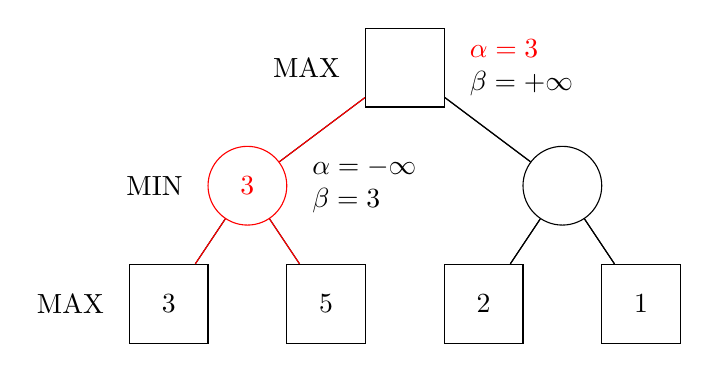
\begin{tikzpicture}[
        level distance=1.5cm,
        level 1/.style={sibling distance=4cm},
        level 2/.style={sibling distance=2cm},
        circleNode/.style={circle, draw, minimum size=1cm, inner sep=0pt},
        squareNode/.style={rectangle, draw, minimum size=1cm, inner sep=0pt}
    ]
        % Root node
        \node[squareNode] (root) {}
            child {node[circleNode, draw=red] (b) {\textcolor{red}{3}}
                child {node[squareNode] (d) {3}}
                child {node[squareNode] (e) {5}}
            }
            child {node[circleNode] (c) {}
                child {node[squareNode] (f) {2}}
                child {node[squareNode] (g) {1}}
            };

        % Labels for alpha and beta
        \node[right=0.7cm, align=left] at (root) {$\textcolor{red}{\alpha = 3}$ \\ $\beta = +\infty$};
        \node[right=0.7cm, align=left] at (b) {$\alpha = -\infty$ \\ $\beta = 3$};

        % Node labels
        \node[left=0.7cm] at (root) {MAX};
        \node[left=0.7cm] at (b) {MIN};
        \node[left=0.7cm] at (d) {MAX};

        % Edges
        \draw[-, draw=red] (root) -- (b);
        \draw[-] (root) -- (c);
        \draw[-, draw=red] (d) -- (b);
        \draw[-, draw=red] (b) -- (e);
        \draw[-] (c) -- (f);
        \draw[-] (c) -- (g);
    \end{tikzpicture}
    \caption{Alpha-beta pruning - step 3}
\end{figure}

\begin{figure}[htbp]\ContinuedFloat
    \centering
    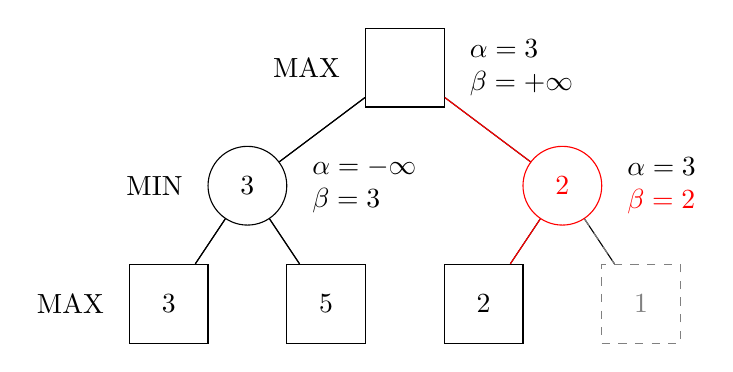
\begin{tikzpicture}[
        level distance=1.5cm,
        level 1/.style={sibling distance=4cm},
        level 2/.style={sibling distance=2cm},
        circleNode/.style={circle, draw, minimum size=1cm, inner sep=0pt},
        squareNode/.style={rectangle, draw, minimum size=1cm, inner sep=0pt}
    ]
        % Root node
        \node[squareNode] (root) {}
            child {node[circleNode] (b) {3}
                child {node[squareNode] (d) {3}}
                child {node[squareNode] (e) {5}}
            }
            child {node[circleNode, draw=red] (c) {\textcolor{red}{2}}
                child {node[squareNode] (f) {2}}
                child {node[squareNode, dashed, gray] (g) {1}}
            };

        % Labels for alpha and beta
        \node[right=0.7cm, align=left] at (root) {$\alpha = 3$ \\ $\beta = +\infty$};
        \node[right=0.7cm, align=left] at (b) {$\alpha = -\infty$ \\ $\beta = 3$};
        \node[right=0.7cm, align=left] at (c) {$\alpha = 3$ \\ $\textcolor{red}{\beta = 2}$};

        % Node labels
        \node[left=0.7cm] at (root) {MAX};
        \node[left=0.7cm] at (b) {MIN};
        \node[left=0.7cm] at (d) {MAX};

        % Edges
        \draw[-] (b) -- (root);
        \draw[-, draw=red] (root) -- (c);
        \draw[-] (d) -- (b);
        \draw[-] (b) -- (e);
        \draw[-, draw=red] (c) -- (f);
        \draw[-, draw=gray, dashed] (c) -- (g);
    \end{tikzpicture}
    \caption{Alpha-beta pruning - step 4}
\end{figure}

\begin{figure}[htbp]\ContinuedFloat
    \centering
    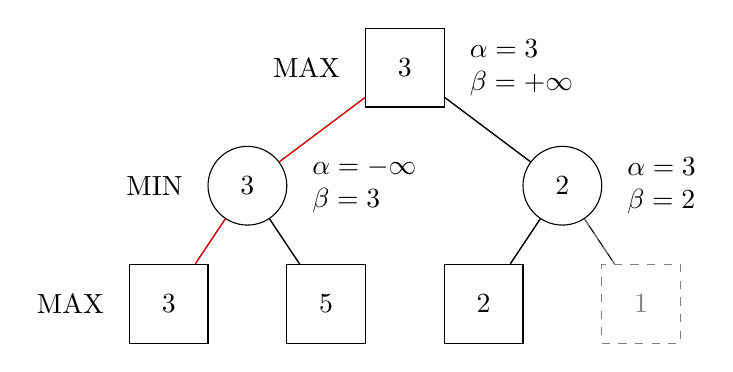
\begin{tikzpicture}[
        level distance=1.5cm,
        level 1/.style={sibling distance=4cm},
        level 2/.style={sibling distance=2cm},
        circleNode/.style={circle, draw, minimum size=1cm, inner sep=0pt},
        squareNode/.style={rectangle, draw, minimum size=1cm, inner sep=0pt}
    ]
        % Root node
        \node[squareNode] (root) {3}
            child {node[circleNode] (b) {3}
                child {node[squareNode] (d) {3}}
                child {node[squareNode] (e) {5}}
            }
            child {node[circleNode] (c) {2}
                child {node[squareNode] (f) {2}}
                child {node[squareNode, dashed, gray] (g) {1}}
            };

        % Labels for alpha and beta
        \node[right=0.7cm, align=left] at (root) {$\alpha = 3$ \\ $\beta = +\infty$};
        \node[right=0.7cm, align=left] at (b) {$\alpha = -\infty$ \\ $\beta = 3$};
        \node[right=0.7cm, align=left] at (c) {$\alpha = 3$ \\ $\beta = 2$};

        % Node labels
        \node[left=0.7cm] at (root) {MAX};
        \node[left=0.7cm] at (b) {MIN};
        \node[left=0.7cm] at (d) {MAX};

        % Edges
        \draw[-, draw=red] (b) -- (root);
        \draw[-] (root) -- (c);
        \draw[-, draw=red] (d) -- (b);
        \draw[-] (b) -- (e);
        \draw[-] (f) -- (c);
        \draw[-, draw=gray, dashed] (c) -- (g);
    \end{tikzpicture}
    \caption{Alpha-beta pruning - step 5}
\end{figure}

\newpage

\noindent Having described the main search algorithms, it is important to explain how the skill of both human and computer chess players is measured. Next, we describe the console communication protocol used by chess engines, and finally, we provide an overview of how \textit{Stockfish} operates internally.

\section{Elo rating system}

The Elo rating system, developed by \textit{Arpad Elo} in the 1960s, is a method used to calculate the relative skill levels of players in two-player games such as chess~\cite{Elo}. It was adopted by the FIDE in 1970 as the main rating system for all federated players.

\vspace{1em}

\noindent Each player has a numerical rating, which increases or decreases based on the outcome of games against other rated players. The core idea is that the difference in ratings between two players predicts the expected outcome of a match.

\vspace{1em}

\noindent The expected score for player \( A \) against player \( B \) is calculated using the formula:

\[
E_A = \frac{1}{1 + 10^{(R_B - R_A)/400}}
\]

where:
\begin{itemize}
  \item \( R_A \) is the rating of player \( A \),
  \item \( R_B \) is the rating of player \( B \),
  \item \( E_A \) is the expected score for player \( A \) (between 0 and 1).
\end{itemize}

\noindent Similarly, the expected score for player \( B \) is \( E_B = 1 - E_A \).

\vspace{1em}

\noindent After a game, the players' ratings are updated using the formula:

\[
R'_A = R_A + K (S_A - E_A)
\]

where:
\begin{itemize}
  \item \( R'_A \) is the new rating of player \( A \),
  \item \( S_A \) is the actual score achieved by player \( A \) (1 for a win, 0.5 for a draw, 0 for a loss),
  \item \( K \) is the development coefficient (often set to 10, 20, or 40 depending on the player's level and federation rules).
\end{itemize}

This system ensures that a player gains more rating points for defeating a higher-rated opponent and loses fewer points when losing to a stronger player.

\section{UCI}\label{sec:uci}

\noindent The chess community has developed an standard console protocol for chess engines to facilitate interoperability between engines and external applications. The \textit{Universal Chess Interface} (UCI)~\cite{UciProtocol} makes it possible to organize games and tournaments between different bots, as well as to integrate engines into graphical user interfaces (GUIs) and other software tools.

\vspace{1em}

\textit{AlphaDeepChess} follows the UCI protocol closely.

\vspace{1em}

\noindent Some of the most used commands are the following:

\begin{itemize}[itemsep=1pt]

    \item \texttt{uci}: tell engine to use the uci interface, the engine must identify itself and sent \texttt{uciok} to acknowledge the uci mode.
    \item \texttt{position [fen <fenstring> | startpos | actualpos] moves <move1> \ldots \\<movei>}: Sets the current position of the board to the FEN string, or applies the list of moves from the starting position or current position. The move format is in long algebraic notation which means sending two squares coordinates like \texttt{e2e4} or \texttt{b1c3}.

    \item \texttt{go}: start calculating on the current position set up with the \texttt{position} command. Some  subparameters are:
    \begin{itemize}[itemsep=1pt]
        \item \texttt{depth <x>}: Specifies the maximum \texttt{depth} to search.
        \item \texttt{movetime <x>}: Specifies the number of \texttt{x} seconds to search. 
    \end{itemize}

    \item \texttt{stop}: stop calculating.
\end{itemize}

\noindent Now that we have covered the fundamental concepts behind chess engines, in the following section we present the most powerful and widely used chess engine.

\section{\textit{Stockfish}}\label{sec:stockfish}

\noindent \textit{Stockfish} is an open source chess engine that has consistently ranked among the strongest in the world~\cite{Stockfish}. It is written in C++ and released under the GNU General Public License (GPL). \textit{Stockfish} has been developed and refined by a large community of contributors.

\vspace{1em}

\noindent \textit{Stockfish} has an estimated Elo rating of around 3644~\cite{StockfishElo}, placing it far above the best human player, Magnus Carlsen, whose peak Elo rating was 2882 in May 2014~\cite{MagnusCarlsenElo}.

\vspace{1em}

\noindent It is based on the minimax search algorithm, enhanced with alpha-beta pruning. In addition, it incorporates several of the techniques described in later chapters (see Chapter~\cref{cap:descripcionTrabajo}).

\vspace{1em}

\par The key component of \textit{Stockfish}'s strength is its use of machine learning algorithms to evaluate chess positions more accurately, in particular, \textit{Stockfish} uses NNUE (Efficiently Updatable Neural Network), a neural network architecture originally developed for shogi engines and later adapted for chess~\cite{NNUE}. NNUE efficiently evaluates positions by finding and learning complex piece patterns. It is optimized to run quickly even on CPUs and significantly improves move ordering (see Chapter~\cref{cap:moveOrdering}), allowing the engine to explore the most promising lines first and prune large parts of the search tree.

\vspace{1em}

In the following section, we describe one of the most popular platforms where both humans and chess engines play competitively.

\section{\textit{Lichess}}\label{sec:lichess}

\textit{Lichess} is a free and open source online chess platform that offers a wide range of features for both casual and competitive players. It was created by Thibault Duplessis in 2010 and has since grown into one of the most popular chess websites in the world, hosting millions of games each day~\cite{Lichess}.

\vspace{1em}

\noindent \textit{Lichess} provides a clean, ad-free user interface. It also features training tools such as puzzles, opening trainers, endgame practice, and access to a large game database.

\vspace{1em}

\noindent One of \textit{Lichess}'s notable features is its use of an Elo based rating system to measure player strength in different game modes. Each player has a separate rating for different time controls and variants.

\vspace{1em}

\noindent \textit{Lichess} also supports chess engines and bots through the \textit{Lichess} Bot API, enabling integration with engines like \textit{Stockfish}. It is often used for engine testing, AI competitions, and research purposes. Many developers and researchers use the \textit{Lichess} platform as a benchmark or interface for evaluating engine performance.

\vspace{1em}

\noindent Finally, the chess community uses specialized tools to evaluate the relative playing strength of chess engines. One of the most widely used tools for this purpose is \textit{Cutechess}.

\section{\textit{Cutechess}}\label{sec:cutechess}

\noindent \textit{Cutechess} is an open source tool widely adopted in the chess programming community. It allows users to run automated matches between engines, compare their performance, and analyze gameplay~\cite{CuteChess}.

\vspace{1em}

\noindent It provides both command-line interface (CLI) and a graphic user interface (GUI), with cross-platform compatibility for Windows, macOS, and Linux. For our purposes, we utilized the CLI version to automate the tests with Python scripts and commands, integrating it into a CI/CD workflow.

\vspace{1em}

\noindent Mainly, this tool is responsible for sending commands to both selected engines via the UCI protocol with parameters such as the search time and depth for each engine, the number of games to play, the time control, or even specific openings to use.

\vspace{1em}

\noindent Then, it manages the games by setting up the board with the \texttt{position} command, sending \texttt{go} to start the search, and stopping when the search time or depth is reached. Moves are alternated between engines so they play against each other automatically. In~\cref{lst:cutechess-example}, we show a \textit{Cutechess} log file, where the starting positions are taken directly from a list of FENs in the \texttt{positions.fen} file.

\begin{lstlisting}[basicstyle=\ttfamily\scriptsize, breaklines=true, frame=single, captionpos=b, caption={Example of \textit{Cutechess}}, label={lst:cutechess-example}]
Running test (8) with the following configuration:
Games: 1, Search Time: 5, Depth: 5
PGN File: results.pgn, EPD File: results.epd, Log File: results.log
Engines: ['AlphaDeepChess', 'Stockfish']
Options: {'Stockfish': {'UCI_LimitStrength': 'true', 'UCI_Elo': '2000'}}
Book: 
Positions: positions.fen
...
 <Stockfish(1): uciok
 >Stockfish(1): setoption name UCI_Elo value 2000
 >Stockfish(1): setoption name UCI_LimitStrength value true
 >Stockfish(1): isready
 <Stockfish(1): readyok
Started game 1 of 1 (AlphaDeepChess vs Stockfish)
 >AlphaDeepChess(0): ucinewgame
 >AlphaDeepChess(0): position fen rnbqkb1r/1p2pppp/p2p1n2/8/3NP3/2N5/PPP2PPP/R1BQKB1R w KQkq - 0 6
 >Stockfish(1): ucinewgame
 >Stockfish(1): setoption name Ponder value false
 >Stockfish(1): position fen rnbqkb1r/1p2pppp/p2p1n2/8/3NP3/2N5/PPP2PPP/R1BQKB1R w KQkq - 0 6
 >AlphaDeepChess(0): isready
 <AlphaDeepChess(0): readyok
 >AlphaDeepChess(0): go movetime 5000 depth 5
 <AlphaDeepChess(0): info depth 1 score cp 130 bestMove c1e3
 <AlphaDeepChess(0): info depth 2 score cp 85 bestMove c1e3
 <AlphaDeepChess(0): info depth 3 score cp 80 bestMove c1e3
 <AlphaDeepChess(0): info depth 4 score cp 62 bestMove c1g5
 <AlphaDeepChess(0): info depth 5 score cp 79 bestMove c1g5
 <AlphaDeepChess(0): bestmove c1g5
 >Stockfish(1): position fen rnbqkb1r/1p2pppp/p2p1n2/8/3NP3/2N5/PPP2PPP/R1BQKB1R w KQkq - 0 6 moves c1g5
 >Stockfish(1): isready
 <Stockfish(1): readyok
 >Stockfish(1): go movetime 5000 depth 5
 <Stockfish(1): info depth 1 seldepth 6 multipv 1 score cp -52 ...
 <Stockfish(1): info depth 2 seldepth 3 multipv 1 score cp -45 ...
 <Stockfish(1): info depth 3 seldepth 3 multipv 1 score cp -39 ...
 <Stockfish(1): info depth 4 seldepth 3 multipv 1 score cp -39 ...
 <Stockfish(1): info depth 5 seldepth 3 multipv 1 score cp -27 ...
 <Stockfish(1): bestmove e7e6
 >AlphaDeepChess(0): position fen rnbqkb1r/1p2pppp/p2p1n2/8/3NP3/2N5/PPP2PPP/R1BQKB1R w KQkq - 0 6 moves c1g5 e7e6
\end{lstlisting}

\noindent In~\cref{lst:cutechess-example}, we set the number of games to $1$, the search time to $5$ seconds, and the search depth to $5$. We also provided a list of starting positions, from which one is chosen at random. Each line starting with \texttt{position fen \ldots} sets the FEN position and adds the moves played.

\vspace{1em}

\noindent Note that both engines stop searching when depth of $5$ is reached and are verified to be ready after \texttt{isready} command.